\documentclass{beamer}
\usepackage[utf8]{inputenc}
\usepackage{hyperref}
\usepackage{multirow}

\title{Computação em Nuvem - Aula 11}
\subtitle{Utilizando - Provedores de computação em nuvem \\
Prof. Me. Juliana Costa-Silva}

\usetheme{lucid}

\begin{document}
\frame{
 \titlepage
}

\frame{
    \frametitle{Roteiro de Aula}
    \tableofcontents
}
%----------------------------------------
\section{Responsabilidades}
\begin{frame}{Responsabilidade}

\begin{center}
	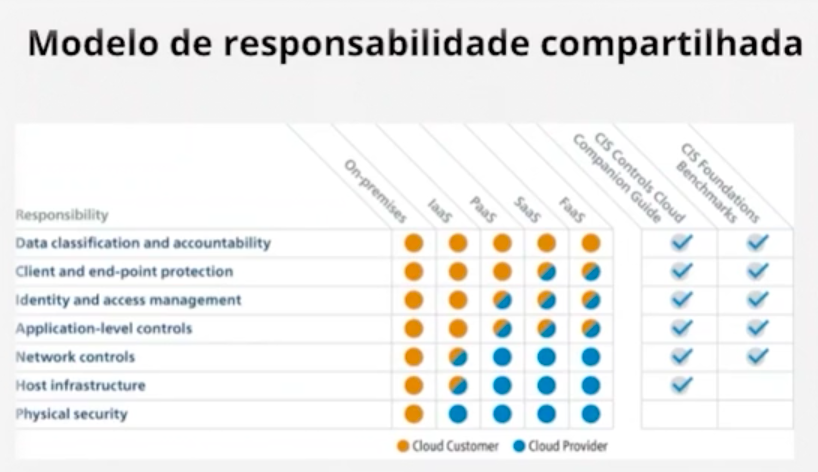
\includegraphics[width=0.85\paperheight]{fig/aula11/responsabilidade.png} \\
	Fonte: \cite{malheiros2019cc}
      \end{center}
    
\end{frame}
%------------------------------------------------
\section{Modelos de cobrança}
\begin{frame}{Modelos de cobrança}

\begin{center}
	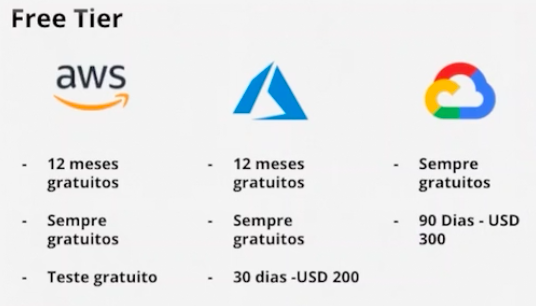
\includegraphics[height=0.65\paperheight]{fig/aula11/cobranca.png} \\
	Fonte: \cite{malheiros2019cc}
      \end{center}
    
\end{frame}
%-------------------------------------------------
\section{Provedores Free}
\begin{frame}{Provedores Gratuitos}
    
   $ \Rightarrow$ \href{https://aws.amazon.com/pt/free/}{Amazon AWS - https://aws.amazon.com/pt/free/} \\
   \vspace{0.5cm}
   $\Rightarrow$ \href{https://cloud.google.com/free}{Google Cloud - https://cloud.google.com/free} \\
   \vspace{0.5cm}
   $\Rightarrow$ \href{https://azure.microsoft.com/pt-br/free/}{Azure - https://azure.microsoft.com/pt-br/free/}
    
\end{frame}
%----------------------------------------
\section{Atividade de aula - PARCIAL}
\begin{frame}{Atividade}
Descreva o funcionamento dos modelos de arquitetura em nuvem:
\begin{enumerate}
    \item Centralizada;
    \item Descentralizada;
    \item Híbrida
\end{enumerate}
\end{frame}

%----------------------------------------
%----------------------------------------
\begin{frame}{Referências}%[allowframebreaks]
 \tiny
 \begin{center}
 	\bibliographystyle{apalike}
	 \bibliography{ref}
 \end{center}
 \end{frame}

\end{document}